\documentclass[a4paper]{article}
%% Sets page size and margins
\usepackage[a4paper,top=3cm,bottom=3cm,left=3cm,right=3cm,marginparwidth=1.75cm]{geometry}
%% Useful packages
\usepackage{amsmath,amsthm,amssymb,amsfonts}
\usepackage{graphicx}
\usepackage[colorinlistoftodos]{todonotes}
\usepackage{bbm}
\usepackage{setspace}
\usepackage{footmisc}
\usepackage{pdflscape}
\usepackage{natbib}
\usepackage{booktabs}
\usepackage{caption}
\usepackage{subcaption}
\usepackage{changepage}
\usepackage{rotating}
\usepackage{bm}
\usepackage{tikz}
\usetikzlibrary{fit,tikzmark}  
\usetikzlibrary{shapes.geometric, arrows}
\usepackage{color, colortbl}

\usepackage{graphicx}
\usepackage[colorlinks=true, allcolors=blue]{hyperref}
\usepackage{url}

\renewcommand\footnotelayout{\fontsize{10}{12}\selectfont}


\tikzstyle{start} = [rectangle, rounded corners, 
minimum width=3cm, 
minimum height=1cm,
text centered, 
draw=black, 
fill=orange!30]

\tikzstyle{process} = [rectangle, 
minimum width=3cm, 
minimum height=1cm, 
text centered, 
text width=3cm, 
draw=black, 
fill=blue!30]

\tikzstyle{stop} = [rectangle, rounded corners, 
minimum width=3cm, 
minimum height=1cm,
text centered, 
draw=black, 
fill=green!30]

\tikzstyle{arrow} = [thick,->,>=stealth]



\interfootnotelinepenalty=10000

\newcommand{\R}{\mathbb{R}}
\newcommand{\N}{\mathbb{N}}
\newcommand{\Z}{\mathbb{Z}}
\providecommand{\C}{\mathbb{C}}

\theoremstyle{definition}
\newtheorem{defin}{Definição}

\theoremstyle{plain}
\newtheorem{theorem}[defin]{Teorema}
\newtheorem{corollary}[defin]{Corolário}

\linespread{2}
\title{Rawls For Electricity Planning Models}

\author{Lauren Beatty\thanks{Environmental Defense Fund  \hspace{.5cm} E-mail: lbeatty1@edf.org \hspace{.5cm}Website: \href{https://lbeatty1.github.io}{https://lbeatty1.github.io}}\\
Matthias Fripp\thanks{Environmental Defense Fund}}

\date{\today}

\begin{document}
\maketitle
\begin{center}
    PRELIMINARY DRAFT - PLEASE DO NOT CITE OR DISTRIBUTE
\end{center}

\begin{abstract}
Renewed interest in the distributional impacts of policies require going beyond typical methods of analysis such as benefit-cost analysis.  In this paper we show how to use least-cost electricity planning models to design equitable systems by modifying their objective functions.  Rather than using the models to minimize costs, we provide the model with a min-max objective function on the distributional health effects of electricity generation and subject the solution to a total cost constraint.  This method provides a menu of plans that equitably reduce pollution exposure.
\end{abstract}


\newpage
\section{Introduction}
Climate change mitigation will require deep cuts to greenhouse gas emissions from the electricity sector.  Least-cost electricity planning models are powerful tools that help policymakers and capacity planners find portfolios of generation technologies that meet reliability requirements and emissions goals.  

However, these models have historically ignored some of the external costs of electricity generation.  
 One major external costs is the generation of local air pollutants.  There is a large body of work on the health effects of air pollution, and a large body of work on the effects of electricity generation on air pollution. 
Air pollution is linked with numerous health impacts such as chronic obstructive pulmonary disease (COPD), acute lower respiratory illness, cerebrovascular disease, ischaemic heart disease, and lung cancer. \cite{Lelieveld2015TheScale} estimate that power generation is linked with 31$\%$ of premature mortality caused by outdoor air pollution in the U.S.

There is also work that has shown that air pollution exposures vary drastically across racial and socioeconomic groups.   \cite{Thind2019FineGeography} find that Black and non-Hispanic white people are exposed to more pollution than other groups and that exposures for low-income people are higher than for high-income people, even after controlling for race.  This highlights the importance for developing planning methods that alleviate rather than reinforce disproportionate burdens.

Previous work has included co-benefits involved with reducing electricity generation from fossil fuels in the objective function \citet{Sergi2020OptimizingBenefits}.
or projected how the electricity transmission might affect the distributional consequences of air pollution exposure \citep{Goforth2022AirStrategies}. However, in this paper, rather than modifying the objective function to include health effects, or use model outputs to project health changes, we endogenize pollution exposure within the electricity model in a way that explicitly considers distributional effects.  This allows us to use the model to produce results that don't unfairly burden certain groups with disproportionate pollution exposure.  It also can be used to answer questions such as "How much can pollution exposure be equitably reduced for $\$100$ billion?" 

This method could also be used to help design electricity transition plans that are equitable in other dimensions.  For example, one concern with the energy transition is that some regions will lose jobs.  This method could help policymakers and planners design electricity systems that avoid causing disruptive employment declines in certain regions. Previous work has linked declines in employment from  coal extraction to negative impacts such as decreases in home values, increases in poverty, and increases in credit utilization and delinquency. Moreover, these studies also suggest that even residents who are not employed by the industry also suffer the negatives consequences associated with the industry's decline (\citet{Kraynak2023TheCountry}, \citet{Blonz2023TheFuels}). 

In this paper, we use

\section{Data}
\subsection{Emissions Data}
Emissions data comes from two sources: EPA's Clean Air Markets Program Data (CAMD) and EPA's National Emissions Inventory (NEI).  The CAMD was created to track compliance with clean air programs, and thus, tracks emissions of CO$_2$, NO$_x$, and SO$_2$.  The NEI was created to track criteria pollutants, criteria precursors, and hazardous air pollutants from \textit{all} sources.  I get emissions of NH$_3$, VOC, and PM2.5 from the NEI. 

\subsection{Power Sector Modelling Inputs}
Stuff about PowerGenome.

\section{Methods}

Least-cost electricity planning models are the gold-standard models used to model capacity expansion in policy.  However, these models tend to have a narrow focus on minimizing costs -- potentially at the expense of distributional concerns.  The energy transition will have wide-ranging effects --such as shifts in the spatial distribution of jobs, or changes in air pollution, that are of interest to policy-makers, but are currently unincorporated into least-cost models.

Previous attempts to consider the health impacts of air pollution have monetized air pollution harms, and inserted them into the cost minimization.  While this is certainly an improvement over not considering these costs at all, this method ignores the fact that inequity in the past has driven current differences in air pollution exposure, and that certain groups may experience higher burdens from air pollution than others.

In this paper, we outline a method to use least-cost electricity planning models to design power systems that produce equitable distributions of air pollution exposure.  We pull inspiration from Rawls and formulate our model as a min-max problem where the social planner minimizes the maximum pollution exposure subject to a cost constraint, rather than minimizing costs.  Running multiple iterations of the model at different cost constraints allows us to understand, how much can we equitably improve air quality and at what costs.
\begin{figure}
    \begin{center}
        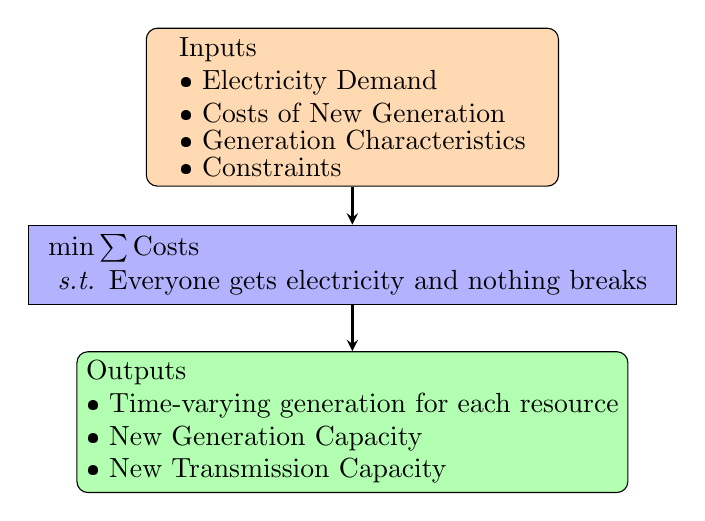
\begin{tikzpicture}[node distance=2cm]
        \node (start) [start, text width=5cm] {\shortstack[l]{Inputs\\• Electricity Demand \\ • Costs of New Generation \\ • Generation Characteristics\\
        • Constraints}};
        
        \node(obj)[process, below of=start, text width=8cm]{\shortstack[l]{$\min \sum \text{Costs}$ \\ \textit{ 
           s.t.   }\text{Everyone gets electricity and nothing breaks }}};
        
        \node (result) [stop, below of=obj] {\shortstack[l]{Outputs\\• Time-varying generation for each resource \\ • New Generation Capacity \\ • New Transmission Capacity}};
        
        \draw [arrow] (start) -- (obj);
        \draw [arrow] (obj) -- (result);
        
        \end{tikzpicture}
    \end{center}
    \caption{Typical Flow of Least-Cost Planning Models}
    \label{fig:enter-label}
\end{figure}


\begin{figure}
\begin{center}
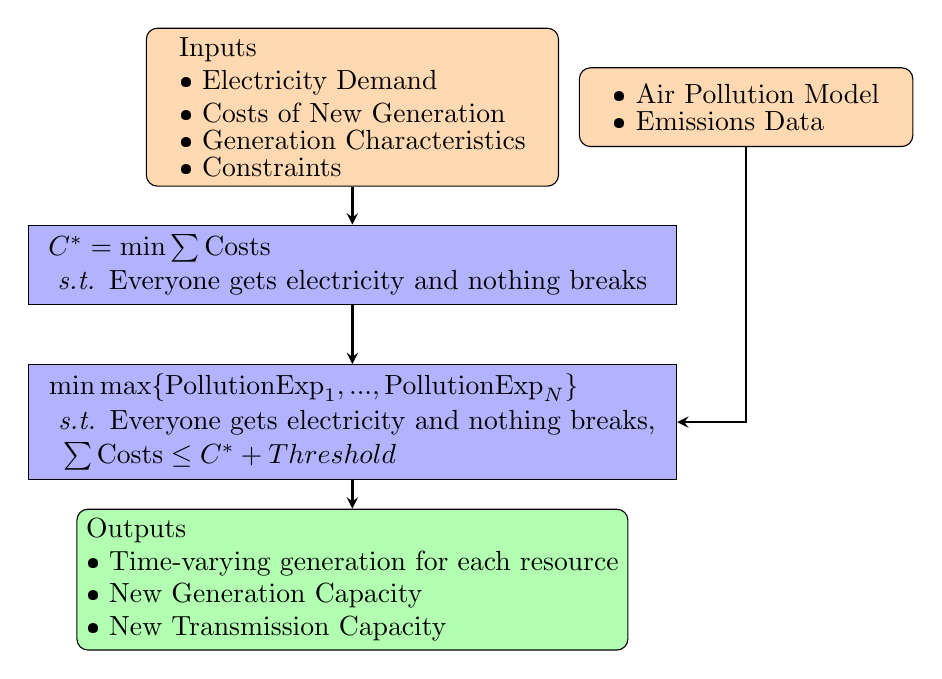
\begin{tikzpicture}[node distance=2cm]

\node (start) [start, text width=5cm] {\shortstack[l]{Inputs\\• Electricity Demand \\ • Costs of New Generation \\ • Generation Characteristics\\
• Constraints}};

\node (air) [start, text width=4cm, right of= start, xshift=3cm] {\shortstack[l]{• Air Pollution Model\\
• Emissions Data}};

\node(obj)[process, below of=start, text width=8cm, xshift=0cm]{\shortstack[l]{$C^* = \min \sum \text{Costs}$ \\ \textit{ 
   s.t.   }\text{Everyone gets electricity and nothing breaks }}};

\node(obj2)[process, below of=obj, text width=8cm, xshift=0cm]{\shortstack[l]{$\min \max\{\text{PollutionExp}_1,...,\text{PollutionExp}_N\}$ \\ \textit{ 
   s.t.   }\text{Everyone gets electricity and nothing breaks,} \\
    $\text{      }\sum \text{Costs} \leq C^*+Threshold$ }};

\node (result) [stop, below of=obj2] {\shortstack[l]{Outputs\\• Time-varying generation for each resource \\ • New Generation Capacity \\ • New Transmission Capacity}};

\draw [arrow] (start) -- (obj);
\draw [arrow] (air) |- (obj2);
\draw [arrow] (obj) -- (obj2);
\draw [arrow] (obj2) -- (result);


\end{tikzpicture}
\caption{Our Modification to the Least-Cost Planning Model}
\end{center}
\end{figure}

\subsection{Air Pollution Modelling}
The end product necessary to endogenize air pollution within electricity planning models are a set of coefficients that describe the marginal effect of a unit of electricity generation on population-weighted mean pollution exposure for different racial groups (though you could also apply the same logic and methodology to differing socio-economic groups more broadly).  

To do this we employ a reduced-form source receptor matrix that that describe the marginal effect of a unit of pollution on downwind concentration of pollution exposure called the InMap Source Receptor Matrix (ISRM).  InMap is a reduced-form emissions to exposure model that uses annual-average parameters to reduce computation complexity relative to a time-resolved chemical transport model. InMap is designed to model annual average PM2.5 pollution exposure, and takes as inputs annual emissions of volatile organic compounds (VOCs), nitrous oxides (NOx), ammonia (NH3), sulfur oxides (SOx), and primary PM2.5.

\section{Results}

\begin{figure}
\centering
\subcaptionbox{Mean empirical emissions rates by technology in tons per MWh.}{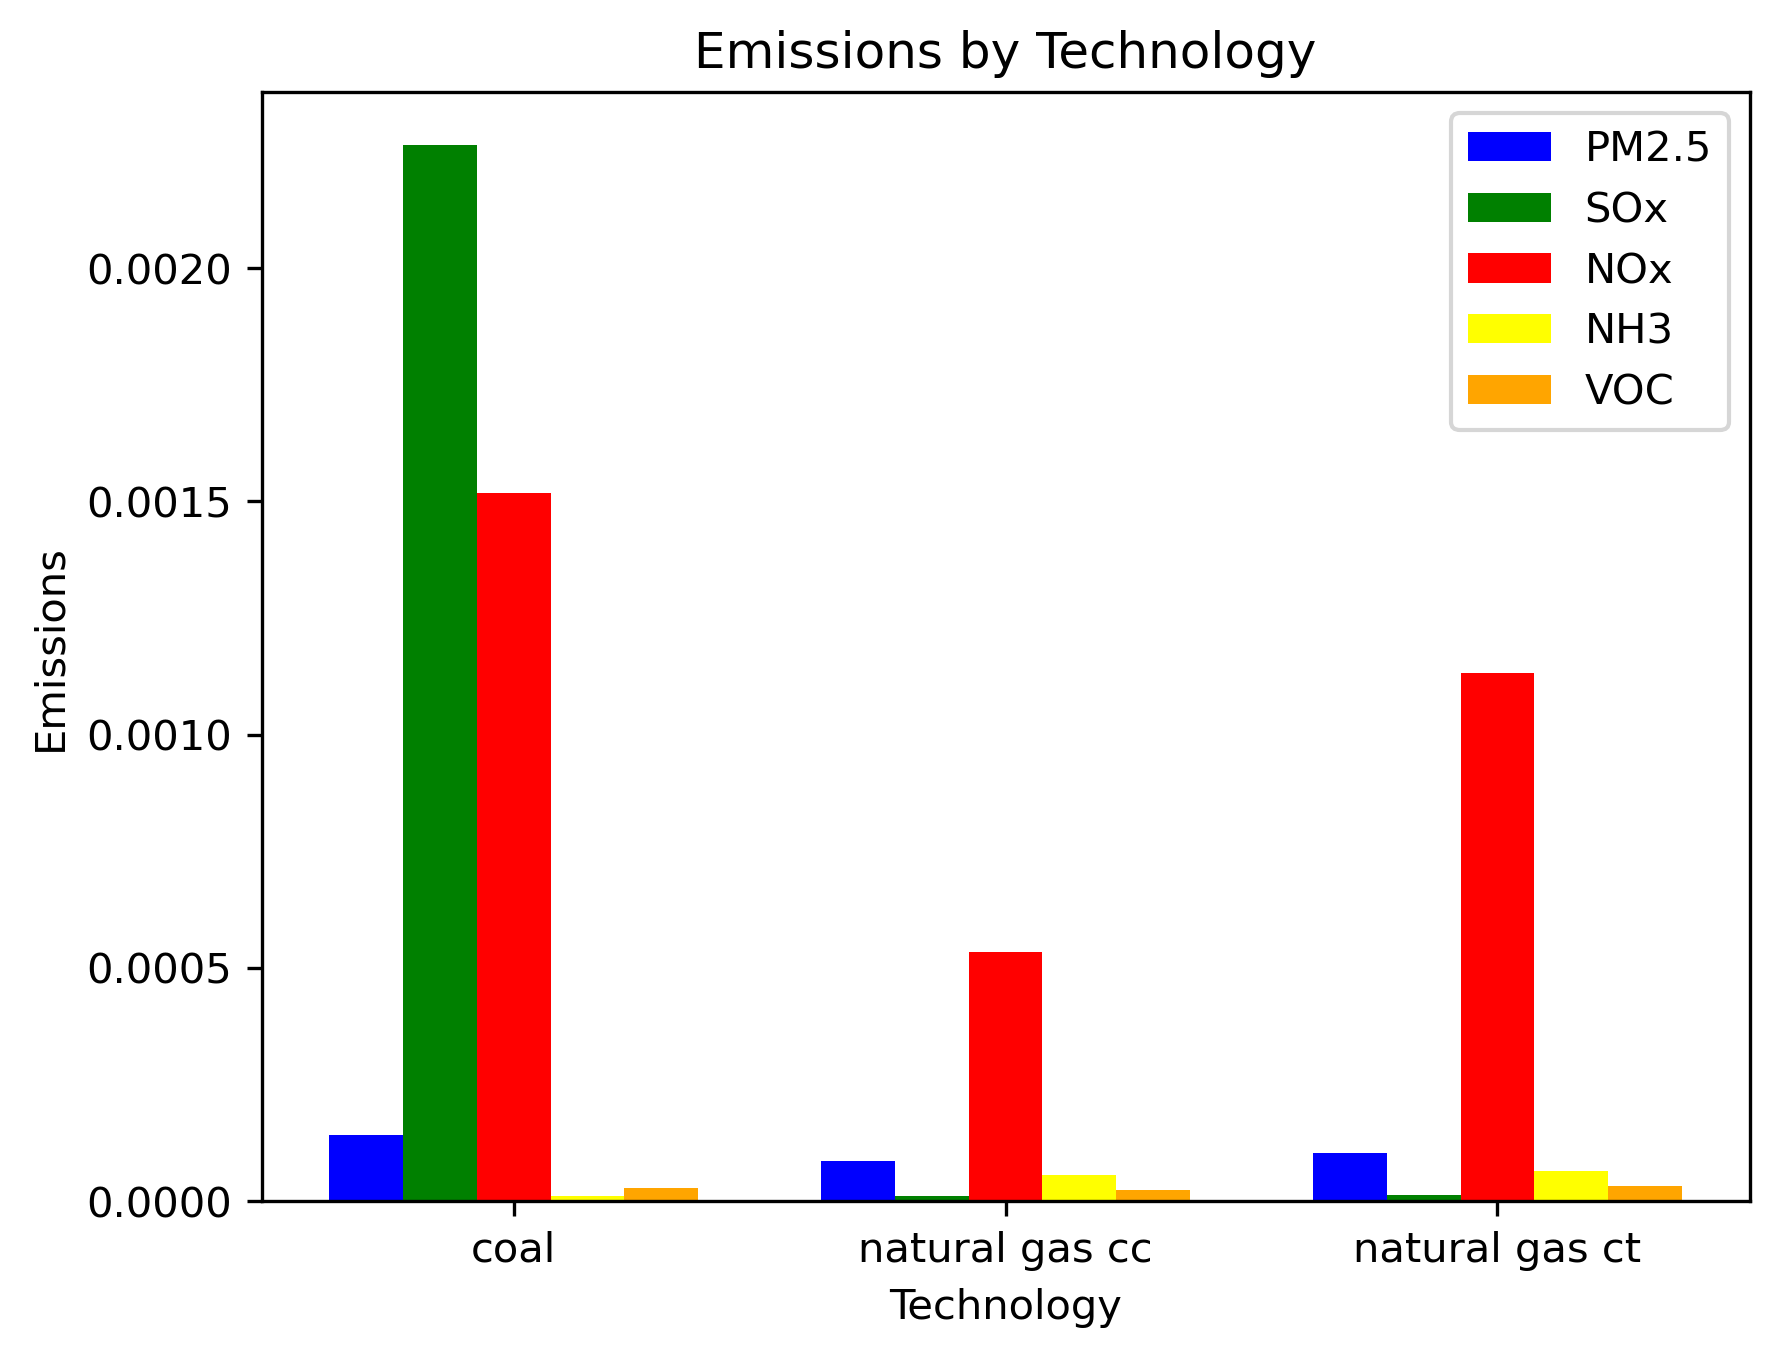
\includegraphics[width=0.45\textwidth]{Figures/EndogenousResults/base_short/base_short_emissions_by_technology.png}}%
\hfill
\subcaptionbox{Mean coefficients describing how a marginal MWh of generation affects mean group-level PM2.5 exposure.}{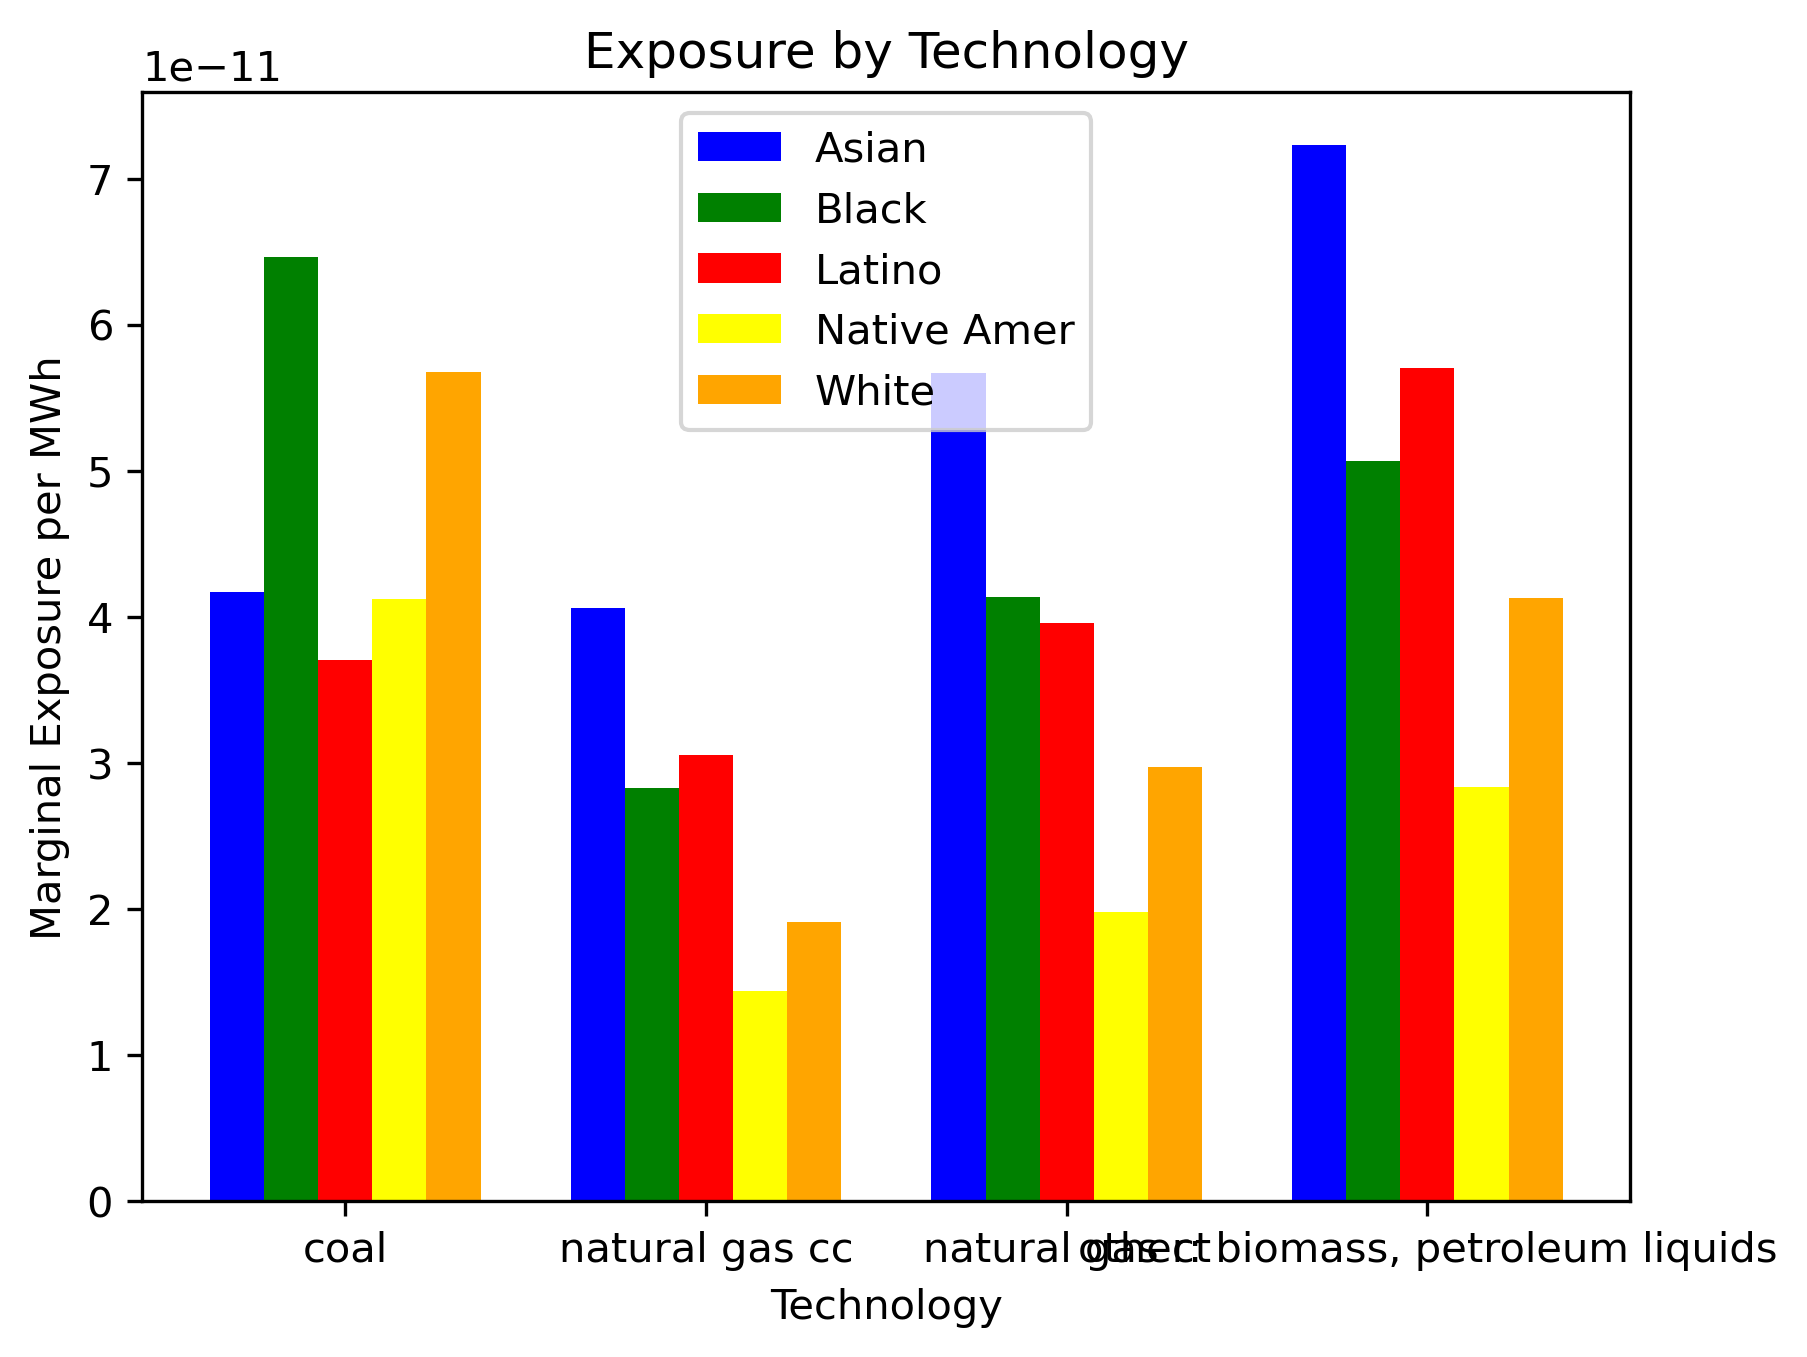
\includegraphics[width=0.45\textwidth]{Figures/EndogenousResults/base_short/base_short_exposure_by_technology.png}}%
\hfill
\caption{Unsurprisingly, coal is far dirtier than other technologies.  However, the discrepancy between technologies is more narrow for exposure.}
\label{EmissionsExposureCoefs}
\end{figure}
In figure \ref{EmissionsExposureCoefs} we plot both average emissions rates, and average exposure coefficients for various technologies.  

\begin{figure}
    \centering
    \includegraphics[width=0.5\linewidth]{}
    \caption{Caption}
    \label{fig:enter-label}
\end{figure}

\begin{figure}
    \centering
    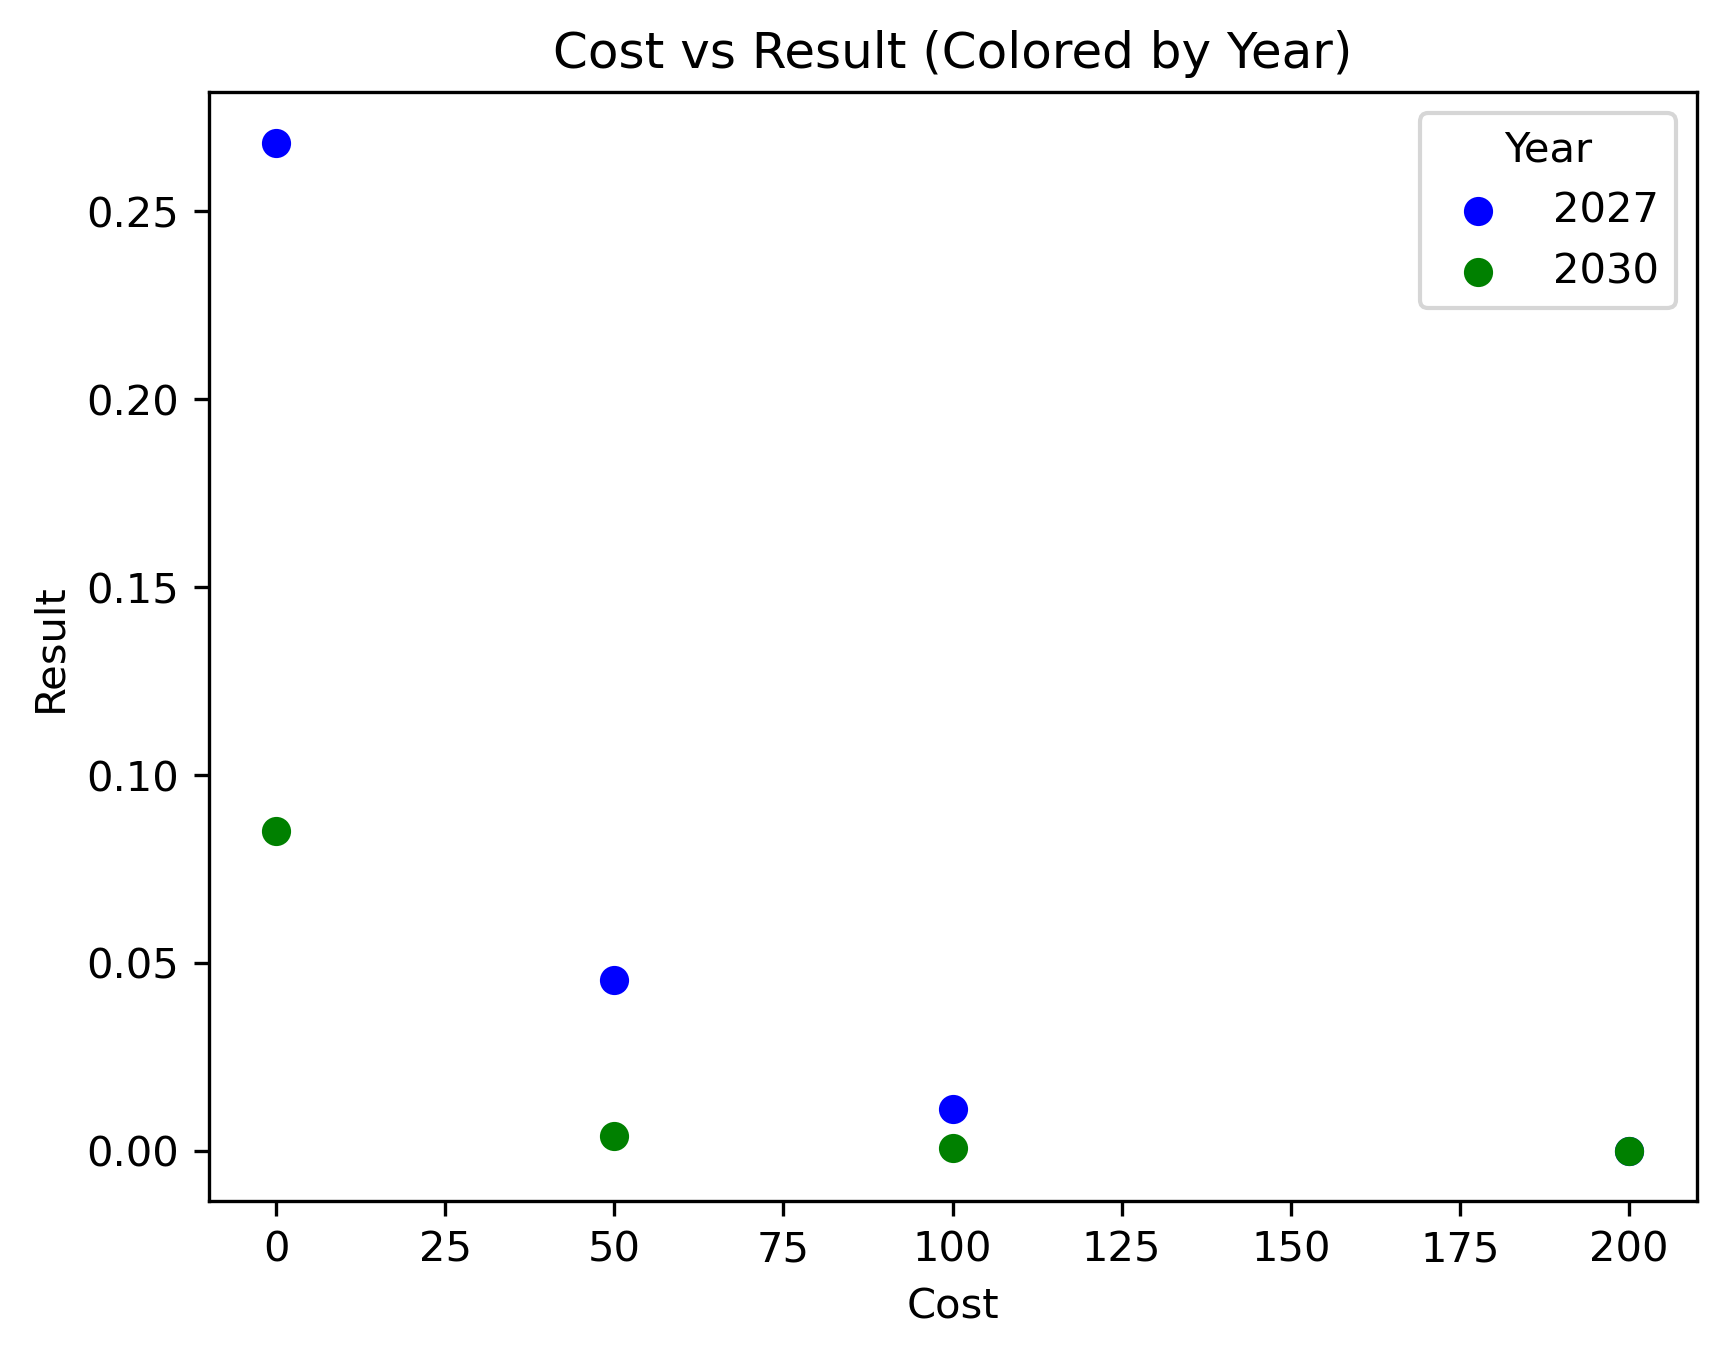
\includegraphics[width=0.7\linewidth]{Figures/EndogenousResults/base_short/exposure_cost_PPF.png}
    \caption{Here we show the relationship between the objective function (min-max of exposure) and the cost limit constraint.}
    \label{PPF}
\end{figure}



\section{Conclusion}


\begin{singlespace}
\newpage
\bibliographystyle{jpe}
%\bibliographystyle{econometrica}
\bibliography{references.bib}
\end{singlespace}

\end{document}